\section{Fundamentals of  Automated Planning}
\label{sec:europa}

{\footnotesize
  \begin{quote}
[Planning] \emph{is an abstract, explicit deliberation process that chooses and
organizes actions by anticipating their expected outcomes. This
deliberation aims at achieving as best as possible some prestated
objectives. Automated planning is an area of Artificial Intelligence
(AI) that studies this deliberation process computationally.} -- from
\textbf{Automated Planning Theory and Practice} by Ghallab, Nau and
Traverso \cite{ghallab04} 
\end{quote}
}

% Planning, for our purposes, can be thought of as determining all the
% small tasks that must be carried out in order to accomplish a goal.
To articulate the fundamentals of automated planning briefly and use
that to motivate the mechanisms we use in our specific form of the
technique we start with a simple example.

\begin{quotation}

  In the near future, a personal robot sets out to buy a gallon of milk
  This involves a number of tasks: obtain keys, obtain wallet,
  start car, drive to store, find and obtain milk, purchase milk, etc.
  The embedded planner has to have a ``model'' of the world in which it
  lives and has to use the task primitives in this model to structure
  the actions so it achieves its goal. Constraints control when certain
  tasks can or cannot occur. For example the robot must obtain the keys
  and wallet \emph{before} driving to the store and pick up the milk
  \emph{before} purchasing it.

\end{quotation}

For such a robot the milk buying plan at the store might look like
\comment{Figure needed}.


% \eu is a general purpose AI planning toolkit developed at NASA Ames.  
% TODO: Talk about NASA missions where \eu has been used.

At the core of the \rx framework, is the deliberation engine, \eu,
which has a rich legacy from NASA missions. \eu is a versatile
Constraint-based temporal planner which continues to be deployed on a
diverse set of applications. We motivate this section with some
problem domains this planner can handle and then delve in substantial
detail.

% \eu is a versatile planning framework.  let's start by looking at some examples of the main problem types that it can tackle.

\paragraph \textit{Constraint Satisfaction}: A canonical problem in
dealing with constraints is the $N$-Queens problem in which chess queens
must be placed on an  $N$x$N$ chessboard so no queens attack the other. Fig.
\ref{fig:nqueens-1} shows an example of a random positioning of queens
on a  $N$x$N$ chessboard. Queens in violation of the non-attack constraint
are highlighted in red.

\begin{figure} \centering
  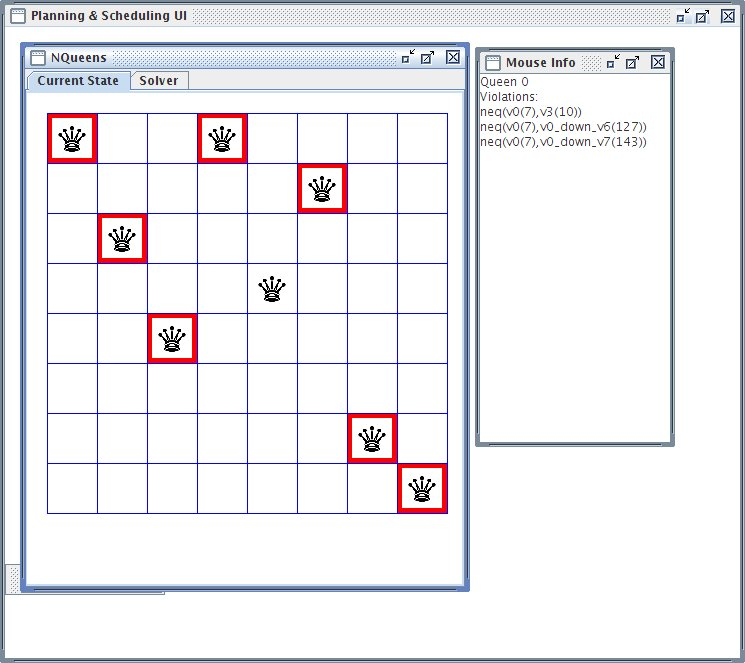
\includegraphics[scale=0.35]{figs/Example-NQueens0.jpg}
  \caption{\small N-Queens problem. Queens in violation of the
    non-attack constraint are highlighted in red.}
\label{fig:nqueens-1}
\vskip+0.1cm
\end{figure}


If we define $N$x$N$ variables Q$_{rc}$, $r \in [1,N]$, $c \in [1,N]$,
Q$_{rc} = 1$ if cell $r,c$ in the chessboard is occupied by a Queen, $0$
otherwise. Then the following constraints need to be satisfied:

\begin{equation}
 Sum(Q_{rc})= \left\{
\begin{array}{l l}
  1 & \forall r \quad \mbox{(only one Queen per row)}\\
  1 & \forall c \quad \mbox{(only one Queen per column)}\\ 
\end{array} \right.
Sum(Q_{r+i,c+i}) = 1\\
Sum(Q_{r-1,c+i}) = 1 \quad \mbox{(only one Queen on each diagonal)}\\
\end {equation} 

\comment{fix newline and numbering problem above}

The problem can be solved by finding assignments for all variables
Q$_{rc}$ that satisfy the above constraints. Fig. \ref{fig:nqueens-2} is
a solution found by \eu using that formulation and a specialized search
procedure.

\begin{figure}
\centering
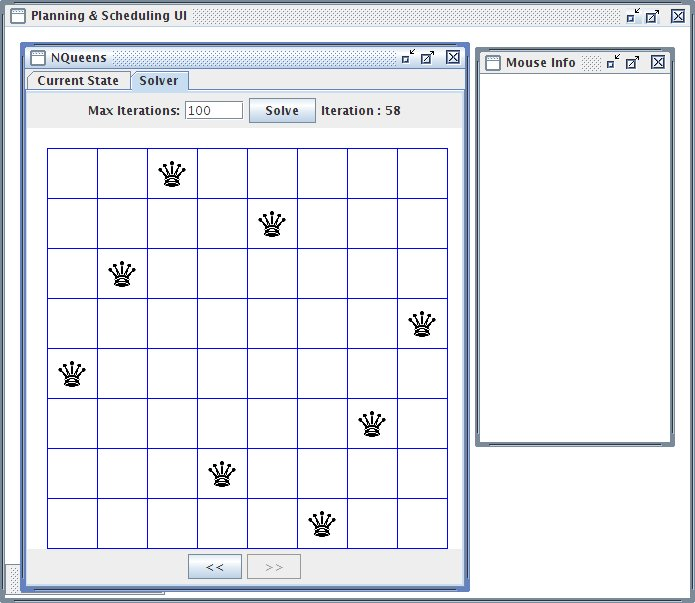
\includegraphics[scale=0.35]{figs/Example-NQueens1.jpg}
\caption{\small N-Queens solution generated by \eu}
\label{fig:nqueens-2}
\vskip+0.1cm
\end{figure}


\paragraph \textit{Scheduling}: In the Resource Constrained Project
Scheduling Problem (RCPSP) \comment{citations needed}, a project
consisting of a set of activities must be scheduled in a way that
satisfies minimum and/or maximum temporal separation constraints. The
activity schedule must also respect fixed limits on the availability of
resources required to perform each activity. In addition to satisfying
temporal and resource constraints, it is common for the user to want to
minimize makespan so that the entire project is finished as early as
possible. Fig. \ref{fig:rcpsp-1} shows an example of a a solution
provided by \eu for an RCPSP instance with 10 activities, 5 resources
and 30 temporal constraints.

\begin{figure}
\centering
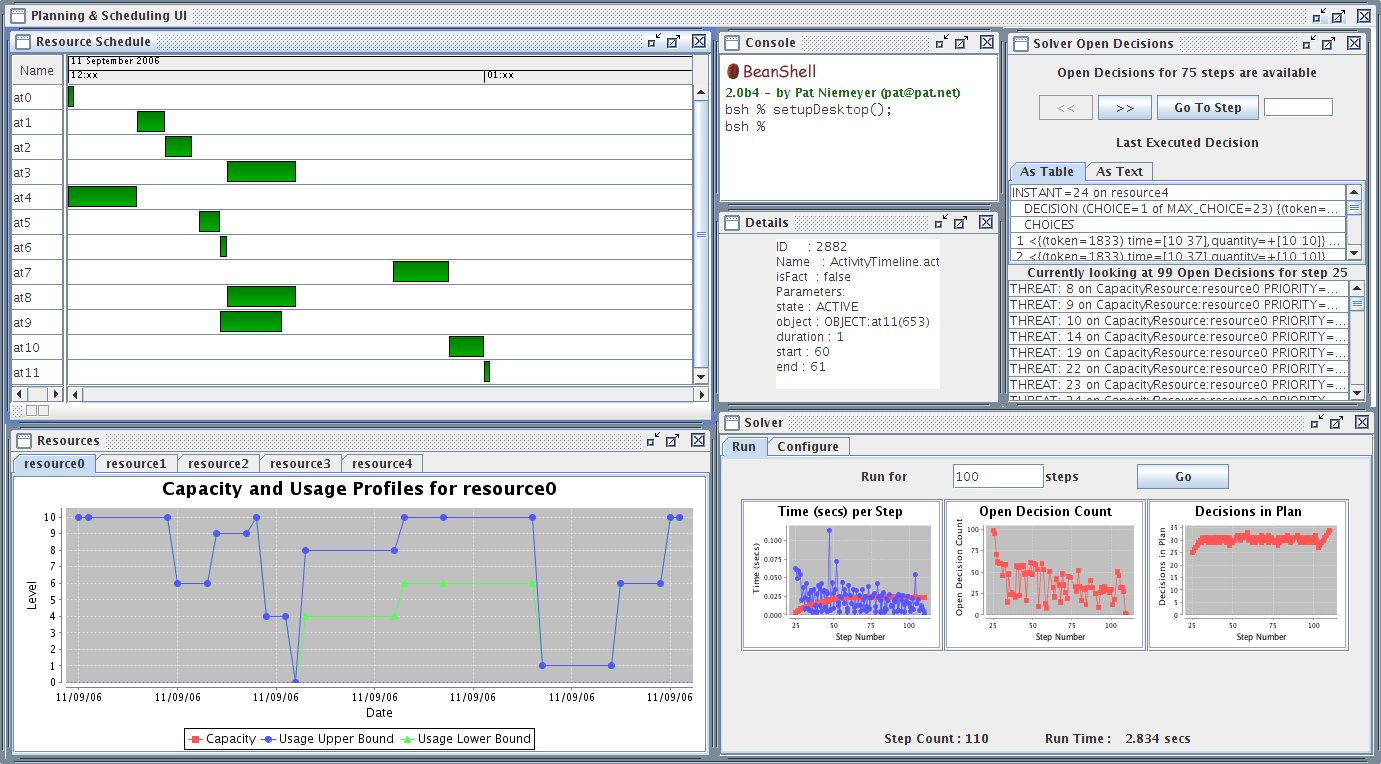
\includegraphics[scale=0.35]{figs/Example-UBO0.jpg}
\caption{\small A \eu solution to an RCPSP \comment{citation} problem.}
\label{fig:rcpsp-1}
\vskip+0.1cm
\end{figure}


\paragraph \textit{Planning}: In the Shopping Agent Problem
\cite{russelnorvig} an agent needs to purchase a set of products (milk,
drill, etc) that are available at specific locations (supermarket,
hardware store, etc), the agent is subject to temporal (must complete
tasks by specific deadlines) and resource (fuel, carrying capacity, etc)
constraints. The agent needs to figure out what actions need to be
performed to find and acquire the required items, as well as when to
perform each of those actions. Fig. \ref{fig:shopping-1} shows a
solution produced by \eu for such a problem instance.

\begin{figure}
\centering
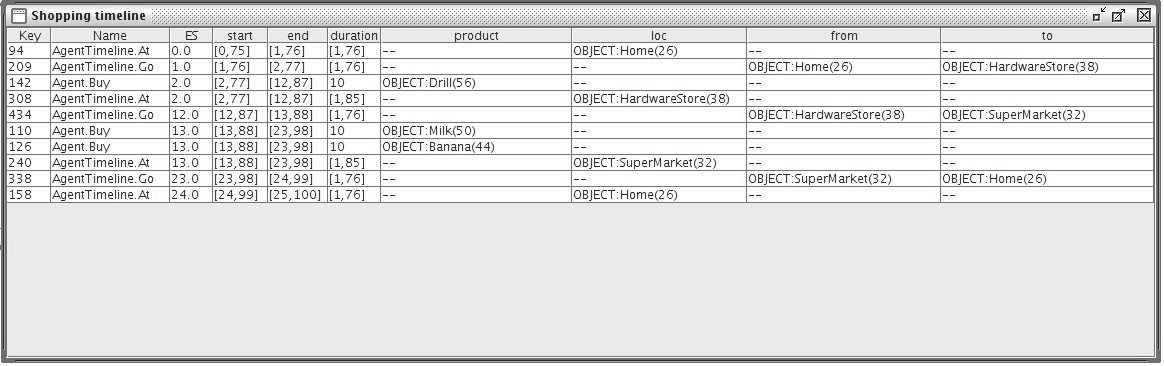
\includegraphics[scale=0.35]{figs/Example-Shopping0.jpg}
\caption{\small A \eu solution to a shopping agent problem domain where
  the agent needs to buy Bananas, Milk and a Drill.}
\label{fig:shopping-1}
\vskip+0.1cm
\end{figure}

As the examples above show, a Planning problem (actions to achieve a
goal) may embed a Scheduling problem (what resources are necessary to
achieve stated goals) and both Planning and Scheduling may embed a
Constraint Satisfaction problem. % since temporal, resource and other
% kinds of constraints must be respected in most real life problems.
The relationships between Planning, Scheduling and Constraint
Satisfaction have been examined \cite{smith00} and have lead to use of
constraint reasoning in \eu as its innermost building block. 

\subsection{Constraint Programming}
\label{sec:europa:cp}

Constraint Satisfaction Programming (also known as Constraint
Programming (CP)) is a discipline that provides a generic framework
for representing, solving and making logical inference on
constraints. A complete treatment of this discipline is given in
\cite{marriott98,apt03} and very concise introductions are provided in
\cite{bartak99,lustig01}.

A constraint programming problem consists of a set of variables $V=
{x_1,..,x_N}$, where each variable takes values from a domain
$d_1,..,d_N$; in this chapter we will deal only with discrete and
finite domains. Given a defined conjunctive set of constraints on the
variables: $C=\{c_1(x_1,..,x_N), ..., c_K(x_1,..,x_N)\}$, the
objective is to find one or more value assignments to $V$ where all
constraints are satisfied. To solve a problem, CP techniques use
logical inference to perform Constraint Propagation, which consists of
two operations:

\begin{enumerate}

\item \textbf{Bounds propagation}: To infer upper and lower variable
  bounds. For example, from the constraints $x_1 + x_2 \leq 2$ \&
  $x_i \geq 0$, we can infer $[0,2]$ bounds for $x_1$ and $x_2$

\item \textbf{Domain reduction}: To infer a valid set of values for a variable.
  For example, for  constraints allDifferent($x_1,x_2,x_3$), $x_i \geq
  0$ \& $x_i \leq 4$, if $x_1 = 1$ and $x_2 = 3$ we can infer that the
  valid domain for $x_3$ is reduced  to $\{2,4\}$

\end{enumerate}

A set of constraints and variables that describe a problem domain are
typically represented as a Constraint Network, where the variables are
nodes and constraints are arcs between the variables. Having this
network representation in mind, a pair of variables $x,y$ is said to be arc consistent if for every
value in $x$'s domain, there is a value in $y$'s domain that is
consistent with all the constraints that connect $x$ and $y$.  A naive
approach to ensuring arc consistency consists of cycling through all
the variable pairs and performing constraint propagation until there
are no variable domain changes. The AC-3 algorithm \cite{mackworth77},
a popular implementation, improves over the naive approach by ignoring
constraints whose variables were not affected since the last
iteration. 

Arc Consistency and other, more stringent consistency definitions can be
used to efficiently prove that a CP problem is unsatisfiable. However,
they generally cannot prove that a CP problem is satisfiable and
provide specific variable assignments that constitute solutions. For
that, search algorithms like global backtracking \comment{citation
  needed} or local search are used; these use consistency as an
efficient way to prune the search space \comment {citation CP
  Handbook}. In theory, solving a CP problem is NP-Hard
\cite{ghallab04}, but often very efficient in practice using a number
of consistency and search algorithms that are well understood.

CP is usually implemented as part of a programming language and
constraints are usually represented as objects \cite{puget95}. Any
constraint that the user is able to reason about can be introduced into the system and, as long as the constraint
propagation protocols specified by the host CP system are enforced, it
will be indistinguishable from any other "primitive'' CP constraint,
such as $\leq$ or $\geq$.

\subsection{Constraint-Based Attribute and Interval Planning}
\label{sec:europa:cp}

The most common planning formulations use a propositional
representation, where the state of the world is represented by a set
of propositions (statements that can be true or false), and operators
change the truth values of these propositions \cite{gen87}. Although
these formulations are powerful and have allowed researchers to
develop numerous contributions in automated planning, there are many
classes of problem domains that are difficult to represent using this
formalism. In particular, it is hard to represent time, resources,
mutual exclusion and concurrency using propositions \comment{citation
  needed}. While CSP representations have traditionally had an edge in
formulating and representing planning problems, 
% It is straightforward to represent and reason about all of
% those elements using a CSP representation, as a result there has been
% some work on doing automated planning while taking advantage of CSP
% (TODO: ref). Traditionally, the entire planning problem is translated
% into a CSP and then solved using traditional CSP methods, this
leading to a formulation where action choices and relationships are
represented as variables and/or constraints, there are at least two
major drawbacks:

\begin{enumerate} 

\item Given that action choices and relationships (rules) are expressed
  through variables, the domain descriptions that result from this
  approach are not intuitive and therefore difficult to understand and
  debug

\item If the structure of a planning model (actions, conditions,
  effects, dependencies at the action level) is not explicitly
  maintained by the CSP planner, the search algorithms are deprived of
  critical information to make better decisions. If that structure is
  maintained (for instance, by internally marking variables that
  represent action choice and relationships between actions), it is
  still hard to write search algorithms as any planning-specific
  insight has to be translated into the CSP representation of
  variables and constraints \comment{For example?}

\end{enumerate}

Constraint-based Planning and specifically Constraint-Based Attribute
and Interval planning (CAIP) \cite{mus94,frank2003} is intended to
close that gap. On one hand, it takes advantage of a CSP
representation; on the other it uses attributes and intervals to
maintain an explicit representation of the elements relevant to
planning. This makes it easier to write algorithms that search for an
reason abut plans. The main elements of CAIP are:

\begin{enumerate}
	\item Intervals: \comment{needs to be defined}
	\item Attributes:
	\item Domain Constraints an Configuration rules:
\end{enumerate}

\comment{Explain how planning problem instances and their solutions are represented}

\subsection{\eu Plan Representation}
\label{sec:europa:pr}

\eu is an implementation of the CAIP framework. 
\comment{once the CAIP section is finished, this section will need an iteration to provide a few pointers back to it}


\textit{Variables} Values that need to be represented to describe the
problem domain and over which we may want to specify constraints. In the Shopping Agent example, the times at which the agent needs to leave or be back, or executes a purchase, are all instances where variables representing time would be used.

\textit{Objects} The things we wish to describe and refer to in a
domain are considered Objects. As in the case with object-oriented
analysis and design, one can seek out the nouns in any domain
description to find likely objects. In the Shopping Agent example, we night consider the Agent itself, Products and Locations all to be objects. Objects have state and behavior. For example, a Shopping Agent can have:
\begin{enumerate}
	\item State: it's location, a bag that contains the products it has already purchased (the bag can in turn be another object), etc.
	\item Behavior: go to a location to look for a product, perform a purchase, return home, etc. 
\end{enumerate}

As in object-oriented design, objects that have similar state and behavior can be described generically in terms of object types or classes. \eu allows the definition of object classes in the same way that it is done in popular object-oriented programming languages. However, to describe state and behavior for the purposes of planning we need a different mechanism, for that we build on the formalism of first order logic as explained below.


\textit{Tokens}

In first order logic, a predicate defines a relation between objects and properties \comment{citation?}. 
In \eu, we define such relations between variables whose domains are sets of
objects and sets of properties to describe state and behavior. For example, we might use a predicate
\texttt{At($a$,$l$)} to indicate that agent
$a$ is at location $l$, or a predicate \texttt{Buy($a$,$p$}) to indicate that agent $a$ is taking acting to buy product $p$. Note that $a$ is a variable which may
have a number of possible values in a problem with multiple
agents. Similarly, $l$ and $p$ are variables whose values are the set of
possible positions and products respectively. \eu can be used to create partial plans, where the domains of variables $a$ and $l$ can have more than one possible value in them, or grounded plans, where single values will be
specified for each variable as we saw in the case of the N-queen's problem.

In general, to come up with an executable plan it is not sufficient to state predicates that describe required state or behavior
without also specifying some temporal extent over which each of those predicates hold. Predicates
that are always true can be thought to hold from the beginning to the
end of time. However, in practice, the temporal extent of interest
must be defined with timepoints to represent its start and end. So we
might want to write \texttt{At($a$,$s$,$e$,$l$)} to indicate that the
agent $a$ is at location $p$ from time $s$ to
time $e$. In fact, this pattern of using such predicates to describe
both state and behavior of objects is so prevalent in \eu that we have
introduced a special construct called a Token which has the built in
variables to indicate the object to which the statement principally
applies and the timepoints over which it holds. In \eu, all predicate
instances are Tokens. Also, in the same way that objects are described generically by classes, in \eu Tokens can be described generically by Token Types.

A Token is an instance of a predicate that represents and object's state or behavior and is defined over
a temporal extent. Every token has five built-in variables:

\begin{enumerate}
    \item \textit {start}: The beginning of the temporal extent over which the predicate
is defined.  
    \item \textit {end}: The end of the temporal extent over which the
predicate is defined.  
    \item \textit {duration}: The constraint \textit{start} + \textit{duration} =
\textit{end} is enforced automatically.  
    \item \textit{object}: The set of objects to
which a token might apply. In a grounded plan each Token applies to a
specific Object, reflecting the intuition that we are using Tokens to
describe some aspect of an Object (i.e. its state or behavior) in
time. However, in a partial plan, the commitment to a specific object
may not yet have been made.
    \item \textit{state}: Tokens can be ACTIVE, INACTIVE, MERGED, or REJECTED. The state
variable captures the token's current state and its reachable states
through further restriction.  This is \eu's mechanism to support CAIP's planning approach, see the Token State Model discussion
below for details.
\end{enumerate}

\comment {resume cleanup here}

\textit{Objects (continued)}

As we have noted, Tokens describe some aspect of an Object in
time. Objects thus may have many Tokens in a plan in order to describe
their state and behavior throughout all points in time of the
plan. Within this general framework, we note a few particulars:

Static Facts: Classes without predicates lead to Objects without
Tokens. This arises where an objects state or behavior is independent
of time. For example, a domain may have a set of locations and/or
paths for which there is nothing more to say than that they exist.

Timelines: Often objects in a domain must be described by exactly one
token for every given timepoint in the plan. Such objects are so
common that we provide a special construct in \eu to extend these
semantics to derived classes. Any instances of a class derived from a
Timeline will induce ordering requirements among its tokens in order
to ensure no temporal overlap may occur among them. See below for
further discussion.

Resources: Metric resources, e.g. the energy of a battery or the
capacity of a cargo hold, are objects with an explicit quantitative
state in time and with a circumscribed range of changes that can occur
to impact that state i.e. produce, consume, use, change. These changes
are captured as tokens. Resources are such a common requirement for
\eu users that special constructs are also provided for
them. Instances of classes derived from a Resource will induce
ordering requirements on their Tokens in order to ensure that the
level of the resource remains within specified limits.

Timelines

It may be sufficient to maintain only a partial-order among
tokens. However, it is often the case that tokens represent states and
actions of a single object in the system. Such tokens are typically
mutually-exclusive. \eu uses a Timeline structure developed in (??)
to concisely capture system components whose behavior is described
over time in this manner.

\comment{This is the first instance that this domain is being
  introduced. Either we need more explanation or it ought to be
  removed.} For example, consider the tire-world domain. The tire was
located in the trunk with the predicate tireLocated(Trunk) and located
on the ground with the predicate tireLocated(Ground). Clearly, the
same tire cannot be in both places at once. A Timeline provides a
simple method for aggregating the statements about a tire such that
they are mutually exclusive.

Figure 1: A Timeline for a Tire

Figure 1 illustrates how a Timeline can be used to describe the
whereabouts of a tire. The tire is an object in the tire-world
represented as a timeline. It has predicates associated with it which
can describe its states and actions over time. The predicate names
need not contain the tire prefix; this is now implicit since the
tokens are assigned to a specific tire instance (i.e. an instance of a
Timeline). While Timelines are a useful element of the \eu planning
paradigm, they are not essential. A more general notion of a system
Object can be used which does not impose restrictions of
mutual-exclusion or non-zero duration. This can be important in
supporting partial-order planning.

For this example, the state of the tire is specified using 3
contiguous tokens. The end and start time-points are related by an
equality constraint. A Moving predicate has been introduced to cover
the transition from one location to another. It takes 2 location
arguments. Notice that precedence relationships exist between tokens
such that they cannot overlap but the start and end times may remain
flexible. To illustrate this, sample times are included. Assume a
total time range of interest between 0 and 1000. In addition, tokens
on Timelines have a minimum duration of 1. As a result the values
shown are the most flexible possible values for the start and end of
each token. There are a number of advantages of allowing this
flexibility. First, the basic structure of the plan can be developed
without over-committing to specific times. If it is not necessary for
the tire to be on the ground at time-step 4, then a planner should not
be forced to specify it. Such an approach permits a least-commitment
approach to planning. Second, in many domains it is simply impossible
to know in planning exactly how long an activity might take. For
example, a common activity of driving a car from one point to another
on a road can take varying amounts of time depending on traffic and
traffic lights. In such circumstances it is more practical to express
upper and lower bounds on durations which naturally lead to intervals
for start and end times. In such domains, flexibility in planning aids
robustness in execution.  Rules

In order for a plan to be valid, it must comply with all rules and
regulations pertinent to the application domain in question. Rules
govern the internal and external relationships of a token. For
example, consider a parameterized predicate describing a transition
from one location to another. Let the parameters be from and to. The
parameters are instantiated on a token as variables whose domain of
values is the set of all locations in a given problem. A rule
governing an internal relationship among token variables might
stipulate that a transition must involve a change in location. This
can be easily expressed as a constraint on the definition of a
predicate of the form: from != to. It is reasonable to further
stipulate that one must be Located somewhere before a transition can
occur, and one must end up Located somewhere when completed. This is
an example of a rule governing an external relationship among
tokens. It specifies a requirement that tokens of the predicate
Located precede and succeed tokens of the predicate Moving.

Figure 2: Internal and external relationships from rules on Moving
Figure 2 illustrates the entities and relations involved in specifying
such a rule on a Moving predicate. The token on which the rule applies
is referred to as the master. Each Located token required by the
master is referred to as a slave. All variables are indicated by name
and their domains are expressed as intervals in the case of temporal
variables and as enumerations for the remainder. Application of a rule
on a token can thus cause slave tokens, variables, and constraints to
be introduced.  Token State Model

The capability of a domain rule to cause a slave token to be created
is a key vehicle through which planning occurs. Semantically, this
rule imposes a requirement for supporting tokens to be in the plan in
order for the master to be valid. There are 2 possibilities to
consider:

The slave is inserted as an active token in the plan. As such, rules
may be activated on the slave, and it may consume resources.

The token is merged with a matching token already in the plan. Once a
slave is merged, the requirement it represents are considered
satisfied. The process of merging passes on all restrictions imposed
on the slave to the active token upon which it is merged. Merging a
token requires finding a target active token that is compatible with
the inactive token. For an active token and an inactive token to be
compatible requires that they are instances of the same predicate and
that no intersections between corresponding variables are empty. The
effect of merging is illustrated in Figure 3.

Figure 3: Merging an inactive token on an active token. Domain
restrictions occur in highlighted variables of active token.

On creation of a token, where the commitment has not been made yet to
activate or merge the token, the token is said to be inactive. There
is a nuance to the state model for tokens which relate to the mode of
its creation. If the token is allocated explicitly by an external
actor, rather than internally through rule firing, it may include the
state rejected indicating the planner is permitted to reject the
token. A valid plan can include rejected tokens. This typically arises
where the token represents a goal that is preferable to achieve but
not mandatory. This state is not reachable for slaves since that would
imply selective adherence to the domain model. Figure 4 presents the
state transition diagram for token states relevant for planning. The
transitions are operations on a partial plan which can decide an
outcome for an inactive token. As operations which may arise in
search, they must be reversible during backtracking. The cancellation
operations in each case are also shown.

Figure 4: Token States and Transitions for Planning

The state of a token is embodied with a 5th and final built-in
variable referred to as the state variable. The planner states are
values in the domain of this variable {MERGED, ACTIVE, REJECTED}. The
INACTIVE state is captured by the variable being unbound. If a value
is removed from the domain, that state will not be reachable. For
example, when a slave is created via a rule, the REJECTED value is
removed from its state variable.  

\textit{Summary}

This has presented the main elements of the EUROPA planning approach. They are:

\begin{enumerate}

\item Temporally scoped predicates and actions (a.k.a. Tokens) to represent
states and actions in time. Note that tokens do not discriminate
between state and action. 

\item Token States which are the basis of planning operations on a partial
plan.

\item Constraints to describe relationships among tokens. This provides an
expressive method of describing interactions among tokens in the
context of Temporal Planning.

\item Timelines as a concise abstraction to express the evolution of state
and behavior for a system component. It provides semantics of mutual
exclusion sequencing in time. Other core abstractions are available in
\eu for handling metric resources.

\item Domain rules to describe internal and external relationships on and
between tokens respectively. Rules are applied to active tokens
(master tokens) referred to as masters and typically produce inactive
tokens (slaves) which are a key vehicle through which the planning
process evolves. The rule structure in \eu differs from the more
restrictive commitment to preconditions and effects in classical
planning which prohibits durative actions and disembodied effects
(i.e. effects which may not occur until some temporal distance after
the end of the action).



\end{enumerate}

